\documentclass[12pt,xcolor=dvipsnames]{beamer}
\usetheme{CambridgeUS}
\usecolortheme{whale}
\setbeamercolor{block title}{use=structure,fg=white,bg=blue!75!black}  
\setbeamercolor{block body}{use=structure,fg=black,bg=blue!5!white}
\setbeamercolor{frametitle}{bg=Blue}

\usepackage{hyperref}   
\usepackage{url}
\hypersetup{urlcolor=red}

\renewcommand{\bibname}{References}
\setbeamertemplate{bibliography item}{[\theenumiv]}

\usepackage{multicol}
\usepackage{verbatim} 
\usepackage{graphics}
\usepackage{graphicx}


%Basic Information
\title{Study and Integration of edX InSight}
\author{Dewang Dinanath Palav}
\date{\today}

%--------------------------------------------------------------------------------------
%               TITLE PAGE (Slide 1)
%--------------------------------------------------------------------------------------
\begin{document}
\begin{frame}
\titlepage
\end{frame}
%--------------------------------------------------------------------------------------


%--------------------------------------------------------------------------------------
%               Outline
%--------------------------------------------------------------------------------------
\begin{frame}
\frametitle{Outline}
\begin{multicols}{2}
\tableofcontents[hideallsubsections]
\end{multicols}
\end{frame}

%--------------------------------------------------------------------------------------
%               Slide 1: Topic 1
%--------------------------------------------------------------------------------------
\section{Introduction}
\begin{frame}[t]
\frametitle{The Project}
\begin{center}
\textit{\large "Knowledge is power"}
\end{center}
\begin{flushright}
-Francis Bacon  
\end{flushright}
\hspace{20pt} The project aims to extract maximum usable data from the huge amount of logs running into terabytes per day, and providing a concise outlook to the educators using edX platform. Using the available technologies a workable product which presents the data in a form easy to analyse. \\

\end{frame}

%--------------------------------------------------------------------------------------
%               Slide 2: Subtopic of Topic 1
%--------------------------------------------------------------------------------------

\subsection{The Motivation}
\begin{frame}[t]
\frametitle{The Motivation}
\hspace{20pt}The concept of e-learning is gaining precedence. With IITBombayX, an indigenous implementation of the edX is pioneering this field. The need for a robust Insight mechanism which analyses the data generated is being felt at large. The ultimate motivation is to meet this need with technology at hand and a contribution to the open source community.
%\begin{center}
%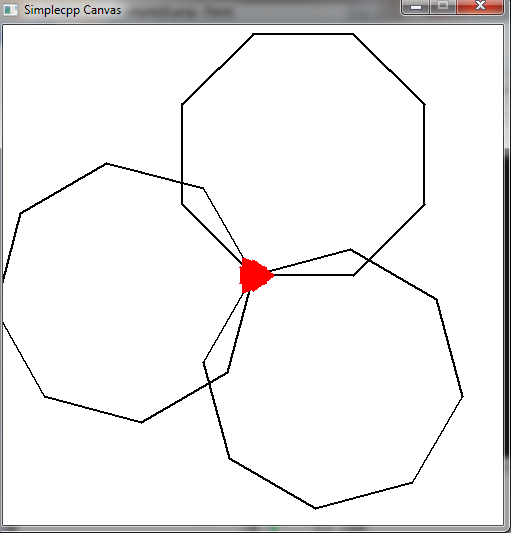
\includegraphics[height=3.5cm]{simple19.png}\\ % Insert your image it this way
%Fig: SimpleCPP Output \cite{SimpleCPP-Windows}
%\end{center}
\end{frame}

%--------------------------------------------------------------------------------------
%               Slide 3: Topic 2
%--------------------------------------------------------------------------------------
\section{Work}
\begin{frame}[t]
\frametitle{Enhancing the present}

Applications:\\
\begin{itemize}
 \item The consistency graph of a student's time of attempting a test gives an insight into the level of seriousness of a student towards a course.\\
 \item A certain extent of dynamic behaviour can be implemented by real time time-per-question statistics.\\
 \item The courses can be personalized to a greater extent by the instructor with the data about the student at hand.\\
\end{itemize}

%\begin{center}
%\begin{tabular}{|c|c|c|}
 %\hline
 %No. & Name & Project \\
 %\hline
 %1 & Firuza & Code::Blocks \\
 %\hline
 %2 & Birundha & edX \\
 %\hline
%\end{tabular}
%\end{center}
\end{frame}

\begin{frame}

\frametitle{The road ahead}

\begin{itemize}
\item The reverse insights to students about the instructors to make a informed choice about the course to be taken and under the instructor of his or her choice.
\end{itemize}
\end{frame}


%---------------------------------------------------------------------------------------
%     Final Slide - References
%--------------------------------------------------------------------------------------
\section{References}
\frametitle{References}
\begin{frame}[allowframebreaks]{References}
\bibliographystyle{ieeetr}
\bibliography{biblio}
\end{frame}
\end{document}
